\documentclass[12pt, a4paper, titlepage, hidelinks]{scrreprt}	
%% UTF-8 File Encoding
\usepackage[utf8]{inputenc}
\usepackage[T1]{fontenc}

%% Language settings
\usepackage[ngerman]{babel}

\usepackage{fullpage}
\usepackage{graphicx}
\usepackage{caption}
\usepackage{subcaption}
\usepackage{placeins}
\usepackage{wrapfig}
\usepackage{url}
\usepackage[raiselinks=true, bookmarks=true, bookmarksopenlevel=1, bookmarksopen=true, bookmarksnumbered=true, hyperindex=true, plainpages=false, pdfpagelabels=true]{hyperref}
\usepackage{fancyhdr}
\usepackage[nottoc]{tocbibind}
\usepackage[usenames, dvipsnames]{color}
\usepackage{xcolor}
\usepackage{textcomp} 
\usepackage{fancybox}
\usepackage{mathtools}
\usepackage{csquotes}
\usepackage{dirtree}

\usepackage{tikz}
\usetikzlibrary{arrows, positioning, fit}

\graphicspath{{images/}}

\usepackage{setspace}
\setstretch{1.4}

\usepackage[a4paper]{geometry}
\geometry{left=3.25cm,right=2.5cm,top=3.5cm,bottom=3.5cm,head=14.5pt,headsep=4ex}

\usepackage[pdftex]{thumbpdf}
\pdfcompresslevel=9

\setcounter{secnumdepth}{3}
\setcounter{tocdepth}{3}

\parindent 0cm
\parskip1.5ex plus0.5ex minus0.5ex
\clubpenalty = 10000
\widowpenalty = 10000
\displaywidowpenalty = 10000

%% Caption configurations
\usepackage{caption}
\DeclareCaptionFont{white}{\color{white}}
\DeclareCaptionFormat{listing}{\colorbox{gray}{\parbox{\textwidth}{#1#2#3}}}
\captionsetup{font=small}
%\captionsetup[lstlisting]{format=listing,labelfont=white,textfont=white}
\definecolor{lightgray}{rgb}{.9,.9,.9}
\definecolor{darkgray}{rgb}{.4,.4,.4}
\definecolor{purple}{rgb}{0.65, 0.12, 0.82}

%% Contents in pdf bookmark list
%% uses etoolbox
\makeatletter
\pretocmd{\tableofcontents}{%
  \if@openright\cleardoublepage\else\clearpage\fi
  \pdfbookmark[0]{\contentsname}{toc}%
}{}{}%
\makeatother

\usepackage{lmodern}

\usepackage[activate={true,nocompatibility},final,tracking=true,kerning=true,spacing=true,factor=1100,stretch=10,shrink=10]{microtype}
\microtypecontext{spacing=nonfrench}

\pagestyle{fancy}
\renewcommand{\chaptermark}[1]{\markboth{\thechapter.\ #1}{}}
\fancyhf{}
\fancyhead[LE,RO]{{\headfont\thepage}}
\fancyhead[LO]{\headfont\nouppercase{\rightmark}}

%% better syntax highlighting
\usepackage[chapter, outputdir=out]{minted}
\usemintedstyle{colorful} %https://raw.github.com/n1k0/SublimeHighlight/master/themes.png
\newcommand{\mintedfileinput}[2]{
\microtypesetup{protrusion=false}
\inputminted[frame=lines,framesep=7pt,linenos=false,numbersep=6pt,baselinestretch=1,xleftmargin=10pt, tabsize=2]{#1}{"../#2"}
\microtypesetup{protrusion=true}
}

\newcommand{\mintedfile}[4]{
\begin{listing}[H]
  \mintedfileinput{#1}{#2}
  \vspace{-16pt}
  \caption{#3}
  \label{#4}
\end{listing}
\vspace{-17pt}
}

\newcommand{\clicommand}[1]{\begin{quote}{\ttfamily \raggedright \noindent #1}\end{quote}}

\hypersetup{
 pdfauthor={Mathias Garbe},
 pdftitle={Projektarbeit Asteroids Dokumentation},
 pdfsubject={},
 pdfkeywords={}
}

\title{Projektarbeit Asteroids}
\subtitle{Dokumentation und Ausblick
\begin{figure}[h!]
  \centering
  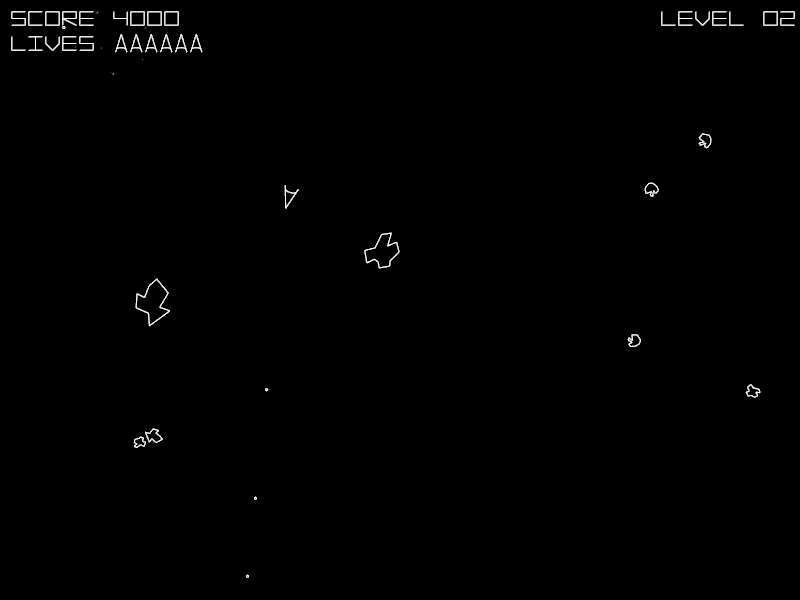
\includegraphics[width=\textwidth]{screenshot.png}
\end{figure}
}
\author{Mathias Garbe}

\begin{document}

\pagenumbering{roman}
\maketitle


\microtypesetup{protrusion=false}
\tableofcontents
\microtypesetup{protrusion=true}

\clearpage

\pagenumbering{arabic}

\chapter{Dokumentation}



\section{Überblick und Ordnerstruktur}

\dirtree{%
.1 /.
.2 cmake \DTcomment{Hilfsskripte für CMake}.
.3 VisualStudio \DTcomment{Visual Studio Solution Template}.
.2 data.
.3 shader \DTcomment{Shader-Quelldateien}.
.2 doc \DTcomment{Dokumentation}.
.3 de.
.2 src \DTcomment{Quelldateien}.
.3 Game \DTcomment{Logik des Spiels}.
.4 Components \DTcomment{Komponenten der Spiel-Entitäten}.
.3 Graphics \DTcomment{Grafik-Subsystem}.
.4 Geometry \DTcomment{Geometrie}.
.4 Shader \DTcomment{Shaderverwaltung}.
.4 Window \DTcomment{Fensterverwaltung}.
.3 Math \DTcomment{Mathe- und Vektorsubsystem}.
}

\section{Abhängigkeiten}

Das Projekt hat folgende Software-Abhängigkeiten:
\begin{itemize}
  \item CMake >=2.8 (Download von \url{http://www.cmake.org})
  \item GLFW >=3.0.4 (Download von \url{http://www.glfw.org})
  \item GLEW >=1.10.0 (Download von \url{http://glew.sourceforge.net})
\end{itemize}

Unter Linux sind diese Abhängigkeiten meist im jeweiligen Paket-Manager verfügbar und einfach zu installieren.

Auch ist ein C++11-fähiger Compiler notwendig. Dies ist unter Linux/Mac OS X \texttt{gcc} in Version 4.7 oder höher sowie \texttt{clang} in Version 3.0 oder höher und unter Microsoft Windows \texttt{Visual Studio 2013} oder höher. Zusätzlich wird noch eine Grafikkarte inklusiver passender Treiber benötigt die mit dem OpenGL 3 Core Profile kompatibel sind.

\section{Buildsystem}
Zum Bauen des Projekts wird CMake verwendet. CMake erzeugt aus den Skriptdatein (\texttt{CMakeFiles.txt}) Makefiles und Projektdateien für eine Reihe von IDEs. Im Zuge der Entwicklung wurde das sowohl mit der Visual Studio Solution, Sublime Text Projekt und GNU Makefiles gearbeitet.  

\subsection{Einrichten von CMake}
\label{cmake-setup}
Für den Fall dass die erforderten Abhängigkeiten nicht mit einem Paketmanager installiert wurden (oder unter Windows entwickelt wird) kann eine \texttt{UserDefinitions.cmake} im Hauptverzeichnis erstellt werden, mit welcher die Pfade von GLFW und GLEW angegeben werden können. Die Datei \texttt{UserDefinitions.cmake.example} kann dabei als Vorlange benutzt werden.

Der Inhalt der \texttt{UserDefinitions.cmake} in einer Windows-Entwicklungsumgebung könnte zum Beispiel so aussehen:

\mintedfile{cmake}{listings/UserDefinitions.cmake.windows}{Ein Beispiel für eine \texttt{UserDefinitions.cmake} unter Windows. Die Windows-Typischen umgekehrten Schrägstriche (Backslash) müssen dabei durch normale Schrägstriche ersetzt werden.}{lst:UserDefinitions.cmake}

Es ist darauf zu achten, dass die \texttt{UserDefinitions.cmake} nicht in die Versionsverwaltung eingecheckt wird, da sie für jede Entwicklungsumgebung spezifisch ist. Deswegen ist diese Datei auch in der \texttt{.gitignore} aufgeführt.

\subsection{Kompilieren des Projekts}
Um die Projektdateien zu bauen öffnet man am einfachsten die Konsole und wechselt in das Projektverzeichnis. Dort können dann mit den folgenden Befehlen die Projektdateien erzeugt werden:
\clicommand{>~mkdir~build\\ >~cd~build\\ >~cmake~..}

Anstatt \texttt{>~cmake ..} zu benutzen kann auch mit \texttt{>~cmake-gui} eine grafische Oberfläche ausgeführt werden, über welche nun CMake eingerichtet werden kann. Falls CMake die Abhänigkeiten GLFW oder GLEW nicht finden kann so wird dies als Fehler ausgegeben und die Ausführung abgebrochen. In diesem Fall muss eine \texttt{UserDefinitions.cmake} erstellt werden oder die Pfadangaben in einer vorhandenen überprüft werde (siehe \autoref{cmake-setup}).

\paragraph{Linux und Mac OS X}
Unter Linux und Mac OS X kann danach per \texttt{>~make} das Projekt gebaut werden. Das Spiel benötigt zum Ausführen Zugriff auf die Shader-Quelldateien, welche sich in \texttt{/data/shader/} befinden. Da das Spiel diese Shader-Dateien relativ zum aktuellen Arbeitsverzeichnis erwartet, muss das Spiel im Hauptverzeichnis gestartet werden:
\clicommand{>~cd ~..\\ >~./build/src/asteroids}

\paragraph{Windows}
Unter Windows kann die erstellte Visual Studio Solution mit Visual Studio 2013 geöffnet und das Projekt gebaut sowie gestartet werden. Die Einrichtung des korrekten Arbeitsverzeichnis hat CMake mithilfe einer Solution Template in \texttt{/cmake/VisualStudio/} übernommen und muss somit nicht von Hand erledigt werden.

\section{Engine-Design}
\subsection{Hauptschleife}

\mintedfile{cpp}{listings/mainloop.cpp}{asdasd}{lst:mainloop.cpp}

\subsection{Fensterverwaltung}
\subsection{Shaderverwaltung}
\subsection{Zeichnen von Geometrie}


\section{Spiel-Design}
\subsection{Komponenten}

Die Spiele-Objekte sind nach einem Komponenten-System entworfen worden. Das bedeutet, das die Objekte nicht von einem oder mehreren Klassen ableiten, welche zum Beispiel Physik und Kollisionen implementieren, sondern eine Referenz auf eine eigene Komponente beinhalten. Damit lassen sich Mehrfachvererbungsprobleme wie das Diamanten-Problem umgehen und gleichzeitig sehr unterschiedliche Objekte realisieren.

Im Moment gibt es nur zwei Komponenten-Typen, die Kollisions- und die Physik-Komponenten. Dieses System ist jedoch variabel und es lassen sich eine Vielzahl von weiteren Komponenten erdenken. So könnte zum Beispiel die Eingabe aus der \texttt{Game}-Klasse gelöst werden und in eine Eingabe-Komponente verschoben werden, welche dann vom Schiff benutzt wird. Auch sind verschieden starke KI-Komponenten für unterschiedliche UFO-Typen oder Schwierigkeitsgerade denkbar. Mit der Einführung einer KI-Komponente könnten selbst Asteroid eine KI erhalten, welche verschiedene Modis ausführen könnte. Zum Beispiel kann ein Asteroid sich um seine eigene Achse drehen, oder generell eine gekrümmte Flugbahn haben. Auch Gravitation könnte so abgebildet werden.

Weitere Anregungen und Erläuterungen sind auch auf GameProgrammingPatterns.com\footnote{\url{http://gameprogrammingpatterns.com/component.html}} und im Blog von Ray Wenderlich\footnote{\url{http://www.raywenderlich.com/24878/introduction-to-component-based-architecture-in-games}} zu finden.

\paragraph{Kollisions-Komponente}
Damit Spielobjekte miteinander Kollidieren können kann jedes Objekt eine Kollisions-Komponente beinhalten. Im Moment gibt es nur eine Komponente, welche zuerst mit einem AABB-Test (Axis-aligned Bounding Box) schnell entscheiden kann, ob eine aufwändigere Linie-zu-Linien Kollision berechnet werden muss. Ist dies der Fall, wird jede Linie jedes Objektes gegen jede Line des anderen Objets miteinander auf einen Schnittpunkt getestet. Mit diesem Verfahren kann eine Pixelgenau Kollision, wie sie im Spiel erforderlich ist, erzielt werden.

\paragraph{Physik-Komponenten}
Für die Physik gibt es zwei unterschiedliche Komponenten. Für alle Objekte, die sich mit einer konstanten Geschwindigkeit bewegen reicht die Genauigkeit einer normalen Eulersche Integration aus. Da jedoch das spielergesteuerte Schiff keine konstante Geschwindigkeit hat und die Richtung sich oft ändert ist die numerische Genauigkeit der Euler-Komponente nicht mehr ausreichend. Dafür gibt es die etwas aufwändiger zu berechnende Runge-Kutta-Komponente, welche eine Runge-Kutta Integration der 4. Ordnung implementiert. Damit wird die Ungenauigkeit auf ein akzeptables Niveau gesenkt welches dem Spieler nicht mehr auffällt.

\chapter{Ausblick}

Diese Kapitel soll einen Ausblick auf Weiterentwicklungs-Potential in dem Engine- und Spieldesign geben.

\section{Portierung auf andere Grafiksysteme}

Das Grafiksystem ist unabhängig vom Spielecode. Alle OpenGL-Befehle werde von der Engine gekapselt, um das Portieren des Spiels auf andere Grafiksysteme wie Mantle oder DirectX zu vereinfachen. Da das Spiel auf OpenGL mithilfe von GLFW für die Fensterverwaltung und Tasteneingabe programmiert wurde befinden sich jedoch innerhalb der Engine Abhängigkeiten darauf. Jedoch wurden keine Konstanten aus OpenGL (wie \texttt{GL\_TRIANGLES} oder ähnliche) benutzt sondern in einem eigenem Enum verpackt.

\mintedfile{cpp}{listings/Mesh.h}{Alle OpenGL-Enums wurden in eigenen Enums verpackt, sodass der Spielecode keine Verweise auf OpenGL hat, hier zu sehen am Beispiel von \texttt{src/Graphics/Geometry/Mesh.h}.}{lst:Mesh.h}

Eine Variante um die Grafikengine auf ein anderes Grafiksystem zu portieren wird in diesem Kapitel vorgestellt. Mithilfe des Pimpl-Idioms (\textit{Pointer to Implementation}) kann das eigentliche Interface welches vom Spielecode benutzt wird unabhängig vom Grafiksystem verwendet werden und das Grafiksystem relativ einfach und schnell ausgetauscht werden, solange dies das Interface voll unterstützt. 

\paragraph{Portierung mithilfe des Pimpl-Idioms}
Anhand der Fensterverwaltung in der Engine kann die Idee des Pimpl-Idioms einfach verstanden werden. Angenommen in der Datei \texttt{Window.h} (siehe Listing \autoref{lst:pimpl/Window.h}) wird das Interface zur Fensterverwaltung definiert und kann so von dem Spielecode benutzt werden.

\mintedfile{cpp}{listings/pimpl/Window.h}{\texttt{Window.h}: Definition des Interfaces ohne eigene Daten. Nur die Referenz auf die eigentliche Implementation ist vorhanden.}{lst:pimpl/Window.h}

Wie man eindeutig sieht hat die Klasse \texttt{Window} keinerlei privaten Daten, die man bei einer Fensterverwaltung erwarten würde. Lediglich ein privater \texttt{unique\_ptr} auf die vorwärts-deklarierte Klasse \texttt{WindowImpl} ist vorhanden. Wenn der Spielecode nun die Datei \texttt{Window.h} inkludiert gibt es keine Möglichkeit auf die internen Daten Einfluss zu nehmen, da die komplette Implementierung in einer noch nicht spezifizierten und auch privaten Klasse liegt.

Erst in der \texttt{Window.cpp} (siehe Listing \autoref{lst:pimpl/Window.cpp}) wird dieser Typ \texttt{WindowImpl} spezifiziert. Je nachdem welches Grafiksytem im Buildsystem ausgewählt wurde werden hier unterschiedliche Implementation angezogen und inkludiert. Da die \texttt{WindowImpl}-Klasse nun spezifiziert ist kann sie auch von der Fensterverwaltung verwendet werden. Im Konstruktor wird eine neue \texttt{WindowImpl}-Instanz erzeugt und als Member initialisiert. Alle Argumente werden der Implementation weitergereicht. Ähnlich werden auch Funktionen wie \texttt{getCursorPosition} einfach auf der eigentlichen Implementation aufgerufen und ggf. der Rückgabewert weitergereicht.

\mintedfile{cpp}{listings/pimpl/Window.cpp}{\texttt{Window.cpp}: Das Interface wrappt sich um eine spezialisierte Implementationsklasse, welche im Konstruktor erstellt wird. Da die Implementation als \texttt{unique\_ptr} angelegt ist muss sich nicht um den Speicher gekümmert werden.}{lst:pimpl/Window.cpp}

Für jedes unterstützte Grafiksystem muss also eine eigene Implementierung programmiert werden, welche dann von dem \texttt{Window} benutzt wird. Dabei ist zu beachten, dass nur eine Implementierung gleichzeitig mit dem Projekt kompiliert werden kann, da alle den gleichen Klassennamen haben.

\mintedfile{cpp}{listings/pimpl/WindowImplGLFW.h}{\texttt{WindowImplGLFW.h}: Ein Beispiel für die Implementierungsdetails der Fensterverwaltung in GLFW. Da dies nicht Teil des öffentlichen Interfaces ist kann es nach belieben und ohne Rücksicht auf Rückwärtskompatibilität verändert werden. Hier als Header-Only-Implementierung zu Darstellungszwecken.}{lst:pimpl/WindowImplGLFW.h}

Weiter Informationen zu dem Pimpl-Idiom befinden sich unter anderem hier:
\begin{itemize}
\item \url{http://www.gotw.ca/gotw/028.htm}
\item \url{http://www.gotw.ca/gotw/024.htm}
\item \url{http://en.wikibooks.org/wiki/C%2B%2B_Programming/Idioms#Pointer_To_Implementation_.28pImpl.29}
\end{itemize}

Das Pimpl-Idiom löst somit einen großen Teil des Portierungsaufwandes, da neue Grafiksysteme hinzugefügt werden können ohne das Interface zu verändern. Somit kann der Spielecode unverändert bleiben. Leider sind das Anfangs erwähnte \texttt{DrawMode}-Enum, welche vom Spielecode benutzt werden, nun immer noch eine direkte Referenz auf die OpenGL-Enums. Dies lässt sich jedoch einfach lösen, indem man im öffentlichen Teil des Interfaces komplett auf die OpenGL-Konstanten verzichtet. Die eigentliche Implementation kann dann selber entscheiden, wie sie damit umgehen möchte. Sie könnte zum Beispiel diese Enums wieder in OpenGL-Konstanten umwandeln, oder mit einer \texttt{switch}-Anweisungen alle Fälle abdecken. 

Jedoch könnte auch argumentiert werden, dass man komplett auf das \texttt{DrawMode}-Enum verzichten sollte und dafür Funktionen wie \texttt{drawTriangles} und \texttt{drawLines} in das Interface einführen sollte. Das löst zwar einige Fälle und eliminiert somit einige Enums, jedoch gibt es zum Beispiel in der Fensterverwaltung (\texttt{src/Graphics/Window}) ein \texttt{Key}-Enum, der alle Tasten auf der Tastatur abbildet. Dieser könnte nur sehr schlecht als Funktionen abgebildet werden und muss dementsprechend erhalten bleiben.

\paragraph{CMake-Unterstützung für mehrere Grafiksysteme}
Da dieses Beispiel auf das Buildsystem angewiesen sind um die Definitionen wie zum Beispiel \texttt{USE\_GLFW} zu setzen, müssen auch die CMake-Skripts angepasst werden. Zum Beispiel könnte dafür eine Option \texttt{graphics-api} eingeführt werden.

\mintedfile{cmake}{listings/CmakeLists-option.txt}{Ein Beispiel wie Optionen der \texttt{CMakeLists.txt} hinzugefügt werden können. Abhängig von den Optionen werden verschiedene Definitionen dem Compiler übergeben und verschiedene Dateien dem Projekt hinzugefügt.}{lst:CmakeLists-option.txt}

Diese Option kann wie folgt mit \texttt{cmake} benutzt werden, hier wird beispielsweise Mantle als Grafiksystem ausgewählt:
\clicommand{>~cmake~-DGRAPHICS-API=MANTLE~..}

\paragraph{Alternativen zum Pimpl-Idiom}
Eine Alternative zu dem Pimpl-Idiom sind \textit{Opaque-Pointer}, oder in Qt auch \textit{D-Pointer} genannt. Dieses Idiom versteckt interne Daten hinter einem anonymen \texttt{struct}, das nur aus der jeweiligen Implementatierung sichtbar ist. 

Genau wie beim Pimpl-Idiom gibt es im Interface wieder keine privaten Daten, außer einen \texttt{unique\_ptr} auf einen forwärts-deklarierten \texttt{struct}.

\mintedfile{cpp}{listings/dpointer/Window.h}{\texttt{Window.h}: Definition des Interfaces ohne eigene Daten. Nur die Referenz auf das private Datenstruct (der D-Pointer oder Opaque-Pointer)ist vorhanden.}{lst:dpointer/Window.h}

Pro Grafikssystem gibt es nun eine Implementierung für dieses Interface. Um trotzdem die erforderlichen, privaten Member zu haben stecken diese nun in einem \texttt{struct}, welches nur in der Implementierung definiert wird.

\mintedfile{cpp}{listings/dpointer/WindowGLFW.cpp}{\texttt{WindowGLFW.cpp}: Private Daten werden im \texttt{WindowDetail} gespeichert, welches nur in dieser Datei sichtbar und zugägnlich ist. Ansonsten wird das komplette Interface in dieser Datei implementiert.}{lst:dpointer/WindowGLFW.cpp}

Das Buildsystem muss sich also darum kümmern die jeweils gewünschte Implementierung zu bauen. Genau wie beim Pimpl-Idiom auch ändert sich das Interface (und somit die Binärkompatibilität) nicht wenn sich die darunterliegende Implementierung ändert oder neue, private Member hinzukommen.

Weiter Informationen zu Opaque-Pointer befinden sich unter anderem hier:
\begin{itemize}
\item \url{http://qt-project.org/wiki/Dpointer}
\item \url{http://en.wikipedia.org/wiki/Opaque_pointer#C.2B.2B}
\end{itemize}

\section{Multithreading}



\end{document}